% Capítulo 3 de la memoria del TFG.
% Archivo previsto: chapters/tecno.tex
% Este capítulo desarrolla el estado del arte y los fundamentos técnicos
% necesarios para comprender el diseño posterior del sistema.

\chapter{Estado del arte}
\label{chap:estado-arte}

Antes de describir el sistema conviene revisar los fundamentos que justifican su enfoque. Construir un RAG jurídico no se reduce a elegir un modelo generativo y hacerle preguntas: hay que localizar la información pertinente, conservar el vínculo de cada fragmento con su norma de origen, ensamblar un contexto útil, redactar una respuesta comprensible y permitir verificar las fuentes. Cada una de esas exigencias sostiene una decisión de diseño posterior.

El capítulo recorre las familias de recuperación de información —léxica, semántica e híbrida—, los modelos de lenguaje y sus límites, la arquitectura \emph{Retrieval-Augmented Generation} (RAG), la fragmentación y la construcción de contexto, la evaluación de estos sistemas y las particularidades del dominio jurídico. Se exponen aquí los conceptos y las alternativas existentes; las decisiones concretas del prototipo llegan en los capítulos siguientes.

\section{Información jurídica y normativa consolidada}
\label{sec:informacion-juridica}

Los documentos jurídicos presentan características que los diferencian de otras colecciones textuales utilizadas habitualmente en sistemas de recuperación de información. Una norma no es solo una secuencia de párrafos: posee una estructura interna formada por títulos, capítulos, artículos, disposiciones, anexos y otros elementos que condicionan su interpretación. Además, cada documento se inserta en un contexto temporal y normativo determinado, por lo que resulta necesario conocer su versión, su vigencia y su procedencia. Esta dimensión temporal es especialmente delicada: una misma norma consolidada agrupa una sucesión de versiones —fruto de sus sucesivas modificaciones, correcciones y derogaciones parciales— y determinar cuál es la redacción vigente en una fecha dada no siempre resulta inmediato, lo que obliga a cualquier sistema de consulta a tratar la versión utilizada y la fecha de captura como información de primer orden.

En el caso de este Trabajo Fin de Grado, la fuente documental principal es la colección de legislación consolidada del \emph{Boletín Oficial del Estado} (BOE). La Agencia Estatal BOE proporciona servicios de datos abiertos para consultar y reutilizar información normativa, incluyendo una API específica de legislación consolidada que permite acceder a metadatos, textos completos, versiones e índices de bloques documentales \cite{boeApiConsolidada}. Esta disponibilidad de datos estructurados resulta especialmente relevante para un sistema RAG, ya que permite preservar información de procedencia y construir enlaces verificables a la fuente oficial.

La consolidación normativa consiste, de forma general, en integrar en un único texto las modificaciones y correcciones expresas que ha recibido una norma desde su publicación original. Su finalidad es facilitar la consulta de la redacción vigente o de versiones anteriores, evitando que el usuario deba reconstruir manualmente la evolución normativa a partir de múltiples disposiciones modificativas. Sin embargo, esta utilidad documental no debe confundirse con valor jurídico propio. El BOE advierte que los textos consolidados tienen carácter informativo y que, para fines jurídicos, debe acudirse a la publicación oficial correspondiente \cite{boeLegislacionActualizada}. EUR-Lex establece una cautela análoga para la legislación consolidada de la Unión Europea, al señalar que la consolidación facilita el acceso a los textos modificados, pero no tiene efectos jurídicos por sí misma \cite{eurlexConsolidation}.

Esta distinción condiciona el alcance de cualquier aplicación basada en estos textos. Un sistema de consulta ciudadana puede ayudar a localizar información normativa, resumirla de forma comprensible y mostrar las fuentes utilizadas, pero no debe presentarse como sustituto de la publicación oficial ni como herramienta de asesoramiento jurídico profesional. En consecuencia, la trazabilidad no es un requisito accesorio: constituye una condición esencial para que el usuario pueda revisar el origen de la información.

Otra dificultad específica del dominio normativo es la distancia entre el lenguaje de la ciudadanía y la redacción formal de las normas: una persona pregunta con vocabulario cotidiano, mientras que el texto emplea expresiones técnicas como ``procedimiento sancionador'', ``extinción del contrato de trabajo'' o ``incapacidad temporal''. Esa distancia justifica estudiar técnicas de recuperación que no dependan únicamente de coincidencias exactas entre las palabras de la consulta y las del documento.

\section{Recuperación de información}
\label{sec:recuperacion-informacion}

La recuperación de información estudia cómo seleccionar, de una colección documental, aquellos elementos que son relevantes para una necesidad de información expresada mediante una consulta. En un sistema de consulta normativa, la colección está formada por documentos legales o por fragmentos derivados de ellos; la consulta es una pregunta formulada por el usuario; y la salida del recuperador es una lista ordenada de evidencias candidatas.

En sistemas RAG la recuperación adquiere una importancia añadida: los documentos seleccionados no son el resultado final, sino la información que condicionará la respuesta del modelo. Si el recuperador omite un fragmento esencial, la respuesta será incompleta; si incluye demasiado ruido, el modelo puede apoyarse en información irrelevante o contradictoria.

Por razones prácticas, el recuperador ordena los resultados y entrega solo los primeros (\emph{top-k}): como la ventana de contexto del modelo es limitada, actúa como un filtro que determina qué partes del corpus llegan a la generación.

Para evaluarla se comparan los documentos recuperados con un conjunto de referencias relevantes mediante métricas como \emph{Recall@k}, \emph{Mean Reciprocal Rank} (MRR) y \emph{Normalized Discounted Cumulative Gain} (nDCG), que capturan, respectivamente, si aparecen suficientes evidencias, si la primera útil llega pronto y si el orden es adecuado.

El cálculo de estas métricas presupone disponer de \emph{juicios de relevancia}: un conjunto de pares consulta--documento etiquetados como relevantes o no relevantes que actúa como referencia (\emph{gold standard}). Construir esos juicios de forma exhaustiva resulta inviable en colecciones de cierto tamaño, por lo que la metodología clásica de evaluación —procedente de la tradición de Cranfield y consolidada en las campañas TREC— recurre al \emph{pooling}: se reúnen los primeros resultados devueltos por varios sistemas y solo se anotan los documentos de ese conjunto común. Esta técnica ahorra esfuerzo, pero arrastra un riesgo conocido. Si el conjunto anotado es pequeño o procede de sistemas poco diversos, los juicios quedan \emph{incompletos} y sesgados a favor de los documentos que esos sistemas ya recuperaban, de modo que un recuperador no representado en la anotación puede quedar injustamente penalizado al recuperar documentos relevantes que nunca llegaron a juzgarse \cite{buckley2004incomplete}. De ahí se derivan dos cautelas metodológicas: conviene construir el conjunto de juicios a partir de sistemas diversos y conviene acompañar toda comparación entre recuperadores de pruebas de significancia estadística que distingan las diferencias reales del ruido del muestreo \cite{smucker2007significance}.

El benchmark BEIR ilustra la diversidad de enfoques de recuperación y la necesidad de evaluar en condiciones heterogéneas. Sus autores comparan modelos léxicos, dispersos, densos, de interacción tardía y de reordenación sobre múltiples conjuntos de datos, y muestran que BM25 continúa siendo una línea base robusta, mientras que algunas técnicas de reordenación pueden mejorar resultados a costa de un mayor coste computacional \cite{thakur2021beir}. En una línea complementaria, el \emph{Massive Text Embedding Benchmark} (MTEB) sistematiza la evaluación de modelos de \emph{embeddings} sobre numerosas tareas e idiomas, y se ha consolidado como una referencia habitual para comparar la calidad de las representaciones vectoriales antes de seleccionar un modelo \cite{muennighoff2023mteb}. Esta observación es relevante para el presente TFG: la recuperación semántica puede resultar atractiva por su capacidad para capturar reformulaciones, pero debe compararse empíricamente con alternativas léxicas e híbridas.

\subsection{Recuperación léxica}
\label{sec:recuperacion-lexica}

La recuperación léxica se basa en la coincidencia entre los términos de la consulta y los términos presentes en los documentos. Su enfoque parte de una intuición sencilla: un documento que contiene palabras relevantes de la consulta tiene más probabilidad de responder a la necesidad de información. Para que esta búsqueda sea eficiente, los sistemas suelen utilizar índices invertidos, estructuras que asocian cada término con los documentos o fragmentos en los que aparece. Antes de construir ese índice, el texto se somete a un \emph{preprocesado lingüístico} que determina qué se considera un «término»: segmentación en unidades léxicas (\emph{tokens}), normalización de mayúsculas y signos, eliminación opcional de palabras vacías (\emph{stopwords}) y reducción de las palabras a una forma común mediante \emph{stemming} o lematización \cite{manning2008ir}. Estas decisiones, en apariencia menores, condicionan qué consultas casan con qué documentos y resultan especialmente sensibles en español, una lengua con flexión morfológica rica.

Uno de los modelos más utilizados en recuperación léxica es BM25. Este método procede del marco probabilístico de relevancia y combina varias señales: la presencia de términos de la consulta, la frecuencia con la que aparecen en un documento, la rareza de esos términos dentro de la colección y una normalización que evita favorecer de forma excesiva a los documentos más largos \cite{robertson2009bm25}. En términos prácticos, BM25 asigna una puntuación más alta a los documentos que contienen términos informativos de la consulta de manera significativa, pero controla el efecto de repeticiones excesivas y de diferencias de longitud. El mismo marco probabilístico admite extensiones para documentos \emph{estructurados en campos} —por ejemplo, para distinguir el título o el encabezado del cuerpo del texto—, como la variante BM25F, que pondera de forma diferenciada las coincidencias según el campo en que aparecen \cite{robertson2009bm25}.

En el dominio jurídico, la recuperación léxica tiene ventajas claras. Muchos conceptos normativos poseen una denominación técnica relativamente estable: ``recurso de alzada'', ``despido disciplinario'', ``incapacidad temporal'', ``silencio administrativo'' o ``protección de datos''. Cuando el usuario emplea esos términos, un método léxico puede localizar con precisión los fragmentos que los contienen. Además, BM25 es interpretable, eficiente y puede ejecutarse adecuadamente en CPU, lo que encaja con entornos locales y reproducibles.

No obstante, la recuperación léxica también presenta limitaciones, pues depende del solapamiento superficial entre consulta y documento: si el usuario pregunta con vocabulario cotidiano y la norma emplea términos técnicos distintos —``silencio administrativo'' frente a ``no me contesta la administración''—, el pasaje relevante puede no recuperarse. Esta diferencia justifica estudiar técnicas semánticas.

Conviene señalar, por último, que la frontera entre lo léxico y lo neuronal se ha difuminado con los modelos de \emph{recuperación dispersa aprendida}, como SPLADE, que emplean redes neuronales para ponderar los términos e incluso expandir el texto con vocabulario relacionado, conservando al mismo tiempo la eficiencia del índice invertido \cite{formal2021splade}. Estos modelos quedan fuera del alcance de este trabajo, pero muestran que la recuperación léxica sigue siendo una línea de investigación activa y no un residuo histórico.

\subsection{Representaciones vectoriales y recuperación semántica}
\label{sec:recuperacion-semantica}

La recuperación semántica busca superar la dependencia exclusiva de coincidencias léxicas. Para ello representa consultas y documentos mediante vectores numéricos, conocidos como \emph{embeddings}, que intentan capturar propiedades semánticas del texto. Si una consulta y un fragmento documental expresan ideas relacionadas, sus vectores deberían situarse cerca en el espacio de representación, aunque no compartan exactamente las mismas palabras.

El uso de embeddings permite formular la recuperación como una búsqueda de vecinos cercanos. La consulta se transforma en un vector y se compara con los vectores de los fragmentos del corpus mediante una medida de similitud, como la similitud coseno o el producto escalar. Los fragmentos más próximos se devuelven como evidencias candidatas. Esta aproximación resulta especialmente útil cuando el usuario emplea expresiones aproximadas, sinónimos o formulaciones diferentes a las contenidas en la norma.

Sentence-BERT introdujo una forma eficiente de obtener embeddings de frases y oraciones mediante arquitecturas siamesas y tripletas, haciendo posible comparar textos mediante similitud coseno con un coste mucho menor que el de comparar todos los pares con un modelo BERT completo \cite{reimers2019sbert}. En recuperación de pasajes, Dense Passage Retrieval (DPR) mostró que los recuperadores densos, basados en codificadores separados para preguntas y pasajes, podían ser competitivos frente a enfoques tradicionales en tareas de preguntas abiertas \cite{karpukhin2020dpr}. Aunque estos resultados proceden de contextos distintos al corpus normativo español, proporcionan el fundamento de la recuperación semántica utilizada en muchos sistemas RAG.

A partir de esas ideas, los modelos de \emph{embeddings} han evolucionado en dos direcciones especialmente pertinentes para una aplicación como la de este trabajo. La primera es la \emph{multilingüalidad}: familias de modelos como E5 multilingüe o BGE-M3 se entrenan sobre numerosos idiomas y alcanzan buenos resultados también en recuperación translingüe, lo que resulta valioso cuando los recursos específicos para una lengua y un dominio —como el español jurídico— son escasos \cite{wang2024me5,chen2024bgem3}. La segunda es el condicionamiento mediante \emph{instrucciones}: en lugar de codificar el texto de forma fija, estos modelos anteponen a la entrada una breve indicación de la tarea —por ejemplo, marcar si el texto es una «consulta» o un «pasaje», o describir el dominio—, de modo que un mismo modelo produce representaciones adaptadas a distintos usos sin necesidad de reentrenarse \cite{su2023instructor}. Ambas propiedades amplían el repertorio de modelos disponibles y, con ello, refuerzan la necesidad de compararlos empíricamente sobre el corpus de destino en lugar de elegirlos por reputación general.

La recuperación semántica presenta ventajas relevantes para una aplicación de consulta ciudadana. Puede recuperar fragmentos relacionados con la intención del usuario aunque la consulta no reproduzca literalmente la terminología jurídica. También permite trabajar con preguntas más naturales, lo que mejora la experiencia de personas no expertas. Sin embargo, no elimina la necesidad de evaluación. Los embeddings pueden recuperar documentos semánticamente cercanos pero insuficientes para responder, pueden confundir conceptos próximos y pueden depender del dominio y del idioma para el que el modelo ha sido entrenado.

Cuando el corpus crece, la búsqueda exhaustiva sobre todos los vectores puede encarecerse; para escalarla suelen emplearse índices vectoriales con búsqueda aproximada, aunque a la escala de este trabajo la búsqueda exacta sigue siendo viable, como se justifica en el capítulo de diseño.

\subsection{Recuperación híbrida}
\label{sec:recuperacion-hibrida}

La recuperación léxica y la recuperación semántica capturan señales diferentes. La primera es fuerte cuando existen coincidencias terminológicas precisas; la segunda es útil cuando la consulta y el documento expresan ideas similares con vocabularios distintos. En dominios especializados, como el jurídico, ambas señales pueden ser complementarias: una consulta puede contener términos técnicos que conviene preservar, pero también reformulaciones ciudadanas que requieren aproximación semántica.

La recuperación híbrida agrupa estrategias que combinan resultados o puntuaciones procedentes de varios recuperadores. Existen distintas formas de realizar esta combinación. Una posibilidad consiste en normalizar las puntuaciones de cada recuperador y calcular una puntuación agregada. Otra consiste en unir las listas de resultados y eliminar duplicados, conservando los documentos mejor posicionados. También puede utilizarse una fusión basada en rankings, donde importa la posición relativa de cada documento en cada lista más que la escala concreta de sus puntuaciones.

Un método conocido para combinar rankings es \emph{Reciprocal Rank Fusion} (RRF). Cormack, Clarke y Büttcher lo propusieron como un procedimiento simple para fusionar resultados de distintos sistemas de recuperación y observaron que podía superar a métodos individuales y a otras estrategias de combinación en los experimentos analizados \cite{cormack2009rrf}. La idea general es favorecer documentos que aparecen en posiciones altas en una o varias listas, sin requerir que las puntuaciones de los recuperadores sean directamente comparables.

Frente a la fusión basada en rangos, otra familia de métodos combina directamente las \emph{puntuaciones} de cada recuperador mediante una \emph{combinación convexa}: una vez normalizadas las escalas —habitualmente con una normalización mínimo--máximo, dado que las puntuaciones léxicas y semánticas no son comparables de partida—, la puntuación final es una media ponderada gobernada por un único parámetro de peso. Un estudio comparativo de funciones de fusión observa que esta combinación convexa, una vez ajustado su parámetro con unos pocos ejemplos, tiende a igualar o superar a RRF tanto dentro como fuera del dominio de entrenamiento, y que RRF, pese a su simplicidad, es sensible a la elección de sus parámetros \cite{bruch2023fusion}. No existe, por tanto, un método de fusión universalmente superior: la elección y el ajuste dependen del corpus y de las consultas, y deben validarse empíricamente.

También existen enfoques híbridos más específicos. Algunos sistemas combinan BM25 con recuperación densa mediante pesos ajustables; otros utilizan recuperación léxica para obtener candidatos iniciales y recuperación semántica para ampliar la cobertura; otros aplican filtros por metadatos antes o después de la búsqueda. La elección depende del corpus, del tipo de consulta, de los recursos disponibles y de la métrica que se quiera optimizar.

\section{Modelos de lenguaje}
\label{sec:modelos-lenguaje}

Los modelos de lenguaje estiman y generan secuencias de texto a partir de patrones aprendidos durante el entrenamiento. Las arquitecturas modernas se basan en el Transformer, que sustituyó las estructuras recurrentes por mecanismos de atención \cite{vaswani2017attention}. Para comprender su papel en un RAG bastan tres nociones: operan sobre unidades llamadas \emph{tokens} (palabras, partes de palabra o signos); generan de forma condicionada por la entrada, las instrucciones y el contexto disponible; y disponen de una ventana de contexto limitada, que impide introducir documentos extensos completos en cada consulta.

Los modelos de gran tamaño han demostrado capacidades notables para seguir instrucciones, resumir información y producir respuestas en lenguaje natural. Brown et al. mostraron que el aumento de escala podía mejorar el rendimiento en múltiples tareas mediante aprendizaje en contexto \cite{brown2020language}. Sin embargo, estas capacidades no implican que el modelo disponga de conocimiento actualizado ni que sus respuestas estén automáticamente fundamentadas en una fuente verificable.

En una arquitectura RAG, el modelo de lenguaje no se utiliza como única fuente de conocimiento. Su función es generar una respuesta a partir de la pregunta del usuario y de las evidencias recuperadas. Esto desplaza parte del problema desde ``qué sabe el modelo'' hacia ``qué documentos se recuperan, cómo se presentan y cómo se controla que la respuesta se apoye en ellos''. Por tanto, el \emph{prompting} no se limita a escribir una pregunta: incluye instrucciones sobre el alcance de la respuesta, el uso de las evidencias, el formato esperado y el comportamiento ante información insuficiente.

Una distinción relevante para este trabajo es la que separa los modelos de \emph{pesos cerrados}, accesibles solo a través de servicios comerciales en la nube, de los modelos de \emph{pesos abiertos}, cuyos parámetros se publican y pueden descargarse y ejecutarse en local. La aparición de familias abiertas competitivas —impulsada de forma destacada por la serie Llama \cite{touvron2023llama2} y continuada por otras como Qwen, Gemma o Mistral— ha hecho viable construir aplicaciones sin depender de \emph{APIs} de pago, lo que mejora la reproducibilidad, elimina el coste por consulta y permite mantener las preguntas dentro de un entorno controlado, una propiedad valiosa cuando se maneja información sensible.

Ejecutar estos modelos en hardware modesto, y en particular sin GPU, plantea un reto de coste computacional. La técnica habitual para afrontarlo es la \emph{cuantización}, que reduce la precisión numérica de los pesos —de 16 a 8 o 4 bits, por ejemplo— y disminuye de forma drástica la memoria y el cómputo necesarios con una pérdida de calidad contenida \cite{frantar2023gptq}. Apoyados en ella, motores de inferencia local como \texttt{llama.cpp}, y las herramientas que los envuelven, como Ollama, permiten servir modelos cuantizados sobre CPU mediante formatos compactos. La elección concreta de los modelos y de su configuración de ejecución se detalla en los capítulos de diseño y experimentos; en este punto basta con constatar que la ejecución local de modelos abiertos constituye hoy una alternativa realista a los servicios comerciales.

\section{Limitaciones de los modelos de lenguaje}
\label{sec:limitaciones-llm}

Los modelos de lenguaje presentan limitaciones relevantes para cualquier aplicación de consulta normativa. La primera es la falta de trazabilidad inherente. Una respuesta puede estar redactada de forma fluida y convincente sin indicar de qué fuente procede cada afirmación. En dominios generales esto ya supone un problema; en el dominio jurídico, donde la fuente y la versión del texto son esenciales, resulta crítico.

La segunda limitación es la posibilidad de generar información incorrecta o no respaldada. La literatura suele referirse a este fenómeno como alucinación, aunque el término agrupa errores distintos: invención de hechos, citas inexistentes, referencias incorrectas, respuestas no fundamentadas o interpretación indebida de documentos. Bender et al. advierten de los riesgos de atribuir a los modelos de lenguaje capacidades de comprensión o veracidad que no se derivan necesariamente de su funcionamiento estadístico \cite{bender2021stochastic}.

La tercera limitación es la actualización del conocimiento. Un modelo entrenado en una fecha determinada no incorpora automáticamente cambios normativos posteriores. Incluso cuando conoce cierta información jurídica, no puede garantizar que corresponda a la versión vigente ni que refleje modificaciones recientes. Esta limitación refuerza la necesidad de utilizar un corpus documental controlado, con fecha de captura y metadatos de procedencia.

La cuarta limitación afecta a la abstención. Un sistema debería ser capaz de indicar que no dispone de información suficiente para responder, especialmente cuando la pregunta se refiere a materias no incluidas en el corpus. El benchmark RGB analiza capacidades relevantes para RAG, entre ellas robustez ante ruido, rechazo negativo, integración de información y robustez contrafactual, y muestra que estas capacidades no pueden asumirse como resueltas por defecto \cite{chen2024rgb}.

En el dominio jurídico, estas limitaciones tienen consecuencias particulares. Dahl et al. analizan alucinaciones jurídicas en modelos de lenguaje y muestran que pueden producir respuestas legalmente incorrectas o referencias problemáticas \cite{dahl2024legalhallucinations}. Magesh et al. estudian herramientas comerciales de investigación jurídica basadas en IA y concluyen que, aunque los sistemas con recuperación pueden reducir ciertos errores frente a modelos generales, no eliminan completamente las alucinaciones ni la necesidad de supervisión y verificación \cite{magesh2025hallucinationfree}. Estas conclusiones no se trasladan directamente al corpus español utilizado en este TFG, pero justifican un diseño prudente: evidencias visibles, enlaces verificables y respuesta explícita cuando el corpus no permite contestar.

\section{Retrieval-Augmented Generation}
\label{sec:rag}

Retrieval-Augmented Generation, o RAG, combina un modelo generativo con una memoria externa formada por documentos recuperables. Lewis et al. proponen esta arquitectura como una forma de combinar memoria paramétrica, contenida en los pesos del modelo, y memoria no paramétrica, representada por una colección documental accesible mediante recuperación \cite{lewis2020rag}. El objetivo es que el modelo no dependa únicamente de lo aprendido durante el entrenamiento, sino que pueda condicionar su respuesta a pasajes concretos recuperados en tiempo de consulta.

Un flujo RAG típico consta de varias etapas. Primero, el sistema recibe una pregunta. Después, un recuperador selecciona documentos o fragmentos relevantes de la colección. A continuación, esos fragmentos se ensamblan en un contexto que se entrega al modelo de lenguaje junto con la pregunta y las instrucciones. Finalmente, el modelo genera una respuesta que debería estar fundamentada en el contexto suministrado. La Figura~\ref{fig:rag-generico} resume este flujo genérico, con sus dos fases —recuperación y generación—.

\begin{figure}[htbp]
    \centering
    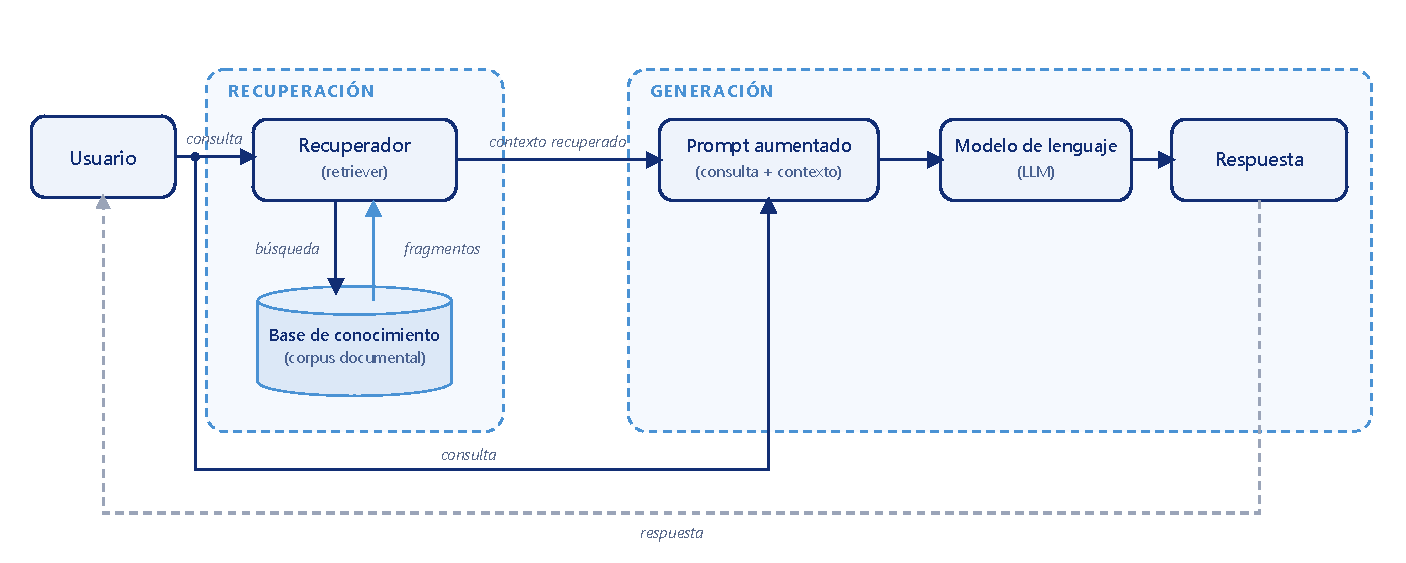
\includegraphics[width=\textwidth]{img/rag_general.pdf}
    \caption{Esquema conceptual de un sistema de generación aumentada por recuperación (RAG). Ante una consulta del usuario, un recuperador selecciona información relevante de una base de conocimiento; ese contexto recuperado se combina con la consulta original en un \emph{prompt} aumentado, a partir del cual un modelo de lenguaje genera la respuesta. Se distinguen las dos fases del proceso: recuperación y generación.}
    \label{fig:rag-generico}
\end{figure}

Esta arquitectura resulta adecuada para la consulta de normativa por varias razones. Permite actualizar el corpus sin reentrenar el modelo generativo, facilita mostrar las fuentes utilizadas y reduce la dependencia del conocimiento paramétrico del modelo. Además, permite separar responsabilidades: el recuperador localiza evidencias; el constructor de contexto selecciona y organiza la información; el modelo redacta la respuesta; y los mecanismos de validación comprueban que la salida respete el formato y las citas esperadas.

Sin embargo, RAG no elimina automáticamente los problemas de los modelos de lenguaje. Si la recuperación falla, el modelo puede no disponer de la información necesaria. Si se recuperan fragmentos ruidosos, puede apoyarse en información irrelevante. Si el contexto es demasiado largo o está mal organizado, puede ignorar partes importantes. Si no se controla la salida, puede citar fuentes inexistentes o presentar afirmaciones no respaldadas. Por ello, los sistemas RAG modernos se estudian como arquitecturas modulares en las que recuperación, generación, reordenación, filtrado, evaluación y observabilidad pueden optimizarse de forma separada \cite{gao2023ragSurvey}.

En este Trabajo Fin de Grado, la arquitectura RAG se adapta a un caso de uso concreto: consulta ciudadana de normativa consolidada. Esto implica tres exigencias adicionales. La primera es conservar la estructura normativa suficiente para que el fragmento recuperado no quede aislado de su artículo o disposición de origen. La segunda es mostrar referencias verificables, preferentemente mediante enlaces oficiales del BOE. La tercera es limitar el alcance de la respuesta, evitando presentar el sistema como una herramienta de asesoramiento jurídico.

\section{Fragmentación documental y construcción de contexto}
\label{sec:fragmentacion-contexto}

Los documentos normativos suelen ser demasiado extensos para introducirse completos en la ventana de contexto de un modelo generativo. Por ello, una etapa habitual en sistemas RAG consiste en dividir los documentos en unidades recuperables. Esta operación, conocida como fragmentación o \emph{chunking}, afecta de forma directa al rendimiento del sistema.

Si los fragmentos son demasiado pequeños, pueden perder información necesaria para interpretar correctamente una disposición. Por ejemplo, un apartado puede depender de una definición anterior, de una excepción o de una condición situada en otro párrafo. Si los fragmentos son demasiado grandes, la recuperación puede volverse menos precisa y el contexto entregado al modelo puede incluir información innecesaria. El equilibrio depende del tipo de documento, de la estructura disponible, del modelo utilizado y del presupuesto de contexto.

En la práctica conviven varias estrategias de fragmentación. Las más sencillas dividen el texto en ventanas de tamaño fijo, a menudo con un solapamiento entre fragmentos consecutivos para no perder información en los límites. Otras buscan cortes más naturales respetando frases o párrafos, o agrupan oraciones por afinidad semántica. Una variante especialmente útil cuando el documento posee estructura es el patrón «recuperar lo pequeño, aportar lo grande» (\emph{small-to-big} o recuperación \emph{padre--hijo}): se indexan unidades pequeñas y precisas para favorecer la exactitud de la recuperación, pero al modelo se le entrega la unidad mayor que las contiene —por ejemplo, el artículo completo— para preservar el contexto necesario. Los sistemas RAG modernos contemplan estas variantes como parte de su diseño modular \cite{gao2023ragSurvey}.

En normativa consolidada, la fragmentación debería respetar, en la medida de lo posible, la estructura jurídica del texto. No es equivalente dividir cada cierto número fijo de palabras que utilizar artículos, apartados o bloques documentales identificados por la fuente. La API de legislación consolidada del BOE ofrece índices de bloques y acceso a textos estructurados, lo que permite diseñar estrategias que aprovechen esa organización documental \cite{boeApiConsolidada}.

La construcción de contexto es la etapa posterior a la recuperación. Su objetivo es transformar los fragmentos recuperados en una entrada útil para el modelo generativo. Esta etapa puede incluir deduplicación, selección de las evidencias mejor posicionadas, expansión con contexto cercano, ordenación, limitación por presupuesto de tokens y asignación de identificadores de evidencia. El orden y la longitud no son indiferentes: se ha observado que los modelos de lenguaje aprovechan mejor la información situada al principio y al final de la entrada que la que queda en mitad de contextos largos, un fenómeno conocido como «\emph{lost in the middle}» \cite{liu2024lostmiddle}, lo que aconseja acotar el tamaño del contexto y situar las evidencias más relevantes en posiciones destacadas. En el dominio jurídico, esta etapa debe preservar la procedencia de cada fragmento para que la respuesta pueda citar evidencias revisables.

La estrategia concreta de fragmentación y construcción de contexto desarrollada en este proyecto se presenta en el capítulo de diseño e implementación. En este capítulo basta con destacar que estas decisiones no son meramente técnicas: condicionan la cobertura, la precisión, la comprensibilidad de la respuesta y la posibilidad de verificar las fuentes.

\section{Generación fundamentada y citas}
\label{sec:generacion-fundamentada-citas}

La generación fundamentada busca que la respuesta del modelo se apoye en evidencias explícitas. En un sistema RAG para normativa, no basta con que la respuesta parezca plausible: debe poder relacionarse con los fragmentos recuperados y con la fuente oficial de la que proceden. Esta exigencia es especialmente importante cuando el usuario no tiene conocimientos técnicos o jurídicos suficientes para detectar errores sutiles.

Las citas cumplen varias funciones. En primer lugar, permiten comprobar la procedencia de una afirmación. En segundo lugar, hacen visible qué documentos han influido en la respuesta. En tercer lugar, ayudan a detectar respuestas incompletas o mal fundamentadas. En cuarto lugar, refuerzan la transparencia del sistema al separar la explicación generada por el modelo de los textos normativos originales.

No obstante, las citas generadas automáticamente también pueden fallar. Un modelo puede citar un fragmento que no respalda realmente la afirmación, puede omitir una evidencia necesaria o incluso inventar identificadores si el sistema no lo impide. Por ello, en aplicaciones RAG no basta con pedir al modelo que cite: es necesario diseñar restricciones, validaciones y formatos de salida que reduzcan la posibilidad de citas no autorizadas.

En este proyecto, la generación fundamentada se relaciona con dos requisitos definidos en el capítulo anterior: asociar las respuestas con referencias verificables a las evidencias utilizadas e impedir que la respuesta cite evidencias no proporcionadas al generador. La implementación concreta de esos mecanismos se explicará más adelante, pero su necesidad se deriva directamente de las limitaciones de los modelos de lenguaje y de las exigencias del dominio jurídico.

\section{Evaluación de sistemas RAG}
\label{sec:evaluacion-rag}

La evaluación de un sistema RAG debe analizar varios componentes. Evaluar únicamente si una respuesta ``suena bien'' no es suficiente. Un sistema puede redactar con fluidez y, al mismo tiempo, recuperar documentos irrelevantes, omitir una norma esencial, citar incorrectamente o responder cuando debería abstenerse.

Una primera dimensión es la calidad de la recuperación. Se pregunta si el sistema localiza evidencias relevantes y si las sitúa en posiciones suficientemente altas. Para ello pueden emplearse métricas de recuperación como \emph{Recall@k}, MRR o nDCG, siempre que exista un conjunto de consultas con evidencias esperadas o juicios de relevancia.

Una segunda dimensión es la calidad de la respuesta. Aquí se analiza si la respuesta contesta a la pregunta, si es comprensible, si mantiene un alcance adecuado y si evita afirmaciones no respaldadas. En una aplicación orientada a ciudadanía, también importa que el lenguaje sea claro y no reproduzca sin más la complejidad de la norma.

Una tercera dimensión es la fundamentación. Evalúa si las afirmaciones de la respuesta están apoyadas por las evidencias citadas. Esta dimensión es crítica en RAG porque la presencia de citas no garantiza por sí misma que las citas sean correctas. RAGAS propone evaluar sistemas RAG considerando aspectos como la relevancia del contexto, la fidelidad de la respuesta al contexto y la calidad de la respuesta generada \cite{es2024ragas}. ARES plantea una evaluación automatizada mediante dimensiones como relevancia del contexto, fidelidad de la respuesta y relevancia de la respuesta \cite{saadfalcon2024ares}.

Muchas de estas dimensiones, especialmente la fidelidad y la corrección, son difíciles de medir con métricas automáticas sencillas porque exigen «entender» el contenido de la respuesta. Una alternativa cada vez más extendida consiste en emplear un modelo de lenguaje potente como \emph{juez} (\emph{LLM-as-judge}) que valore la salida de otro modelo \cite{zheng2023judge}. Este enfoque escala la evaluación y se correlaciona razonablemente con el juicio humano, pero arrastra sesgos documentados: el juez puede verse influido por la posición de las respuestas, por su longitud o por una preferencia hacia textos de su propio estilo (sesgo de auto-preferencia) \cite{zheng2023judge}. De ahí dos cautelas habituales: utilizar como juez un modelo de familia distinta a la del generador, para mitigar la auto-preferencia, y validar sus veredictos frente a anotación humana —por ejemplo, midiendo el acuerdo con el coeficiente $\kappa$ de Cohen \cite{cohen1960kappa}— antes de confiar en ellos. Conviene además recordar que el propio $\kappa$ se comporta de forma engañosa cuando una de las categorías es muy poco frecuente: es la conocida «paradoja de $\kappa$», por la que un acuerdo observado alto puede convivir con un valor de $\kappa$ paradójicamente bajo \cite{feinstein1990paradox}. Como esa situación es habitual en evaluación —por ejemplo, cuando los casos de error o de abstención son escasos—, se han propuesto coeficientes de acuerdo más estables ante el desbalance de clases, como el AC1 de Gwet \cite{gwet2008ac1}, cuyo uso resulta recomendable junto al de $\kappa$. Sin esa validación, las puntuaciones de fidelidad y corrección deben considerarse provisionales.

Estas propuestas son útiles como marco conceptual, pero no sustituyen a una evaluación diseñada para el dominio concreto. La de este trabajo será \textbf{modular} —medirá cada componente por separado, de modo que un fallo pueda atribuirse a su causa real y no quedarse en una nota global que no indica dónde mejorar— y prestará atención especial a las preguntas fuera del corpus, ante las que el sistema debe reconocer que no dispone de información suficiente para responder.

\section{Procesamiento del lenguaje natural en el dominio jurídico}
\label{sec:nlp-juridico}

El procesamiento del lenguaje natural aplicado al Derecho se ocupa de tareas como clasificación de documentos, extracción de información, recuperación jurídica, predicción de resultados, análisis de contratos y apoyo a la investigación legal. El dominio jurídico presenta dificultades propias: terminología especializada, textos largos, estructura formal, importancia de las referencias, cambios normativos y consecuencias potencialmente relevantes de los errores.

LexGLUE es un benchmark de comprensión del lenguaje jurídico que reúne varios conjuntos de datos para evaluar modelos en tareas legales. Sus autores destacan que la utilidad de los modelos depende de su capacidad de generalizar en el dominio jurídico y muestran que los modelos adaptados al dominio pueden ofrecer mejoras frente a modelos generales en distintas tareas \cite{chalkidis2022lexglue}. LegalBench, por su parte, recopila tareas de razonamiento jurídico elaboradas de forma colaborativa con participación interdisciplinar, con el objetivo de evaluar qué tipos de razonamiento legal pueden realizar los modelos de lenguaje \cite{guha2023legalbench}. Conviene subrayar que tanto LexGLUE como buena parte de estos bancos de pruebas se centran en el inglés; los recursos equivalentes para el español jurídico —corpus anotados, modelos especializados o conjuntos de evaluación— son comparativamente escasos, lo que refuerza el interés de apoyarse en modelos multilingües de propósito general y en una evaluación construida específicamente para el corpus del proyecto.

El presente TFG no pretende abordar el razonamiento jurídico general ni resolver tareas complejas como predicción judicial, interpretación doctrinal o análisis jurisprudencial. Su alcance es más delimitado: facilitar la consulta ciudadana de normativa consolidada procedente del BOE mediante recuperación documental y generación fundamentada. Por tanto, las referencias a benchmarks jurídicos sirven para contextualizar la especificidad del dominio, no para afirmar que el sistema resuelve el conjunto de tareas evaluadas en ellos.

La orientación ciudadana introduce una dificultad adicional: el usuario puede no conocer la terminología normativa. La siguiente tabla muestra ejemplos simplificados de esta diferencia entre formulación ciudadana y posible redacción técnica.

\begin{table}[htbp]
\centering
\caption{Ejemplos de distancia entre consulta ciudadana y terminología normativa}
\label{tab:consulta-ciudadana-terminologia}
\begin{tabular}{p{0.43\textwidth}p{0.47\textwidth}}
\hline
\textbf{Consulta ciudadana aproximada} & \textbf{Conceptos o formulaciones normativas relacionadas} \\
\hline
``¿Qué pasa si la Administración no me contesta a tiempo?'' & Silencio administrativo, plazo máximo para resolver y notificar, efectos estimatorios o desestimatorios. \\
``¿Cuánto tiempo tengo para recurrir una resolución administrativa?'' & Plazo de interposición del recurso, recurso de alzada y de reposición, notificación administrativa. \\
``¿Puedo acceder a información que tiene un organismo público?'' & Derecho de acceso a la información pública, límites y causas de inadmisión, transparencia. \\
``¿Pueden tratar mis datos personales sin mi consentimiento?'' & Bases de licitud del tratamiento, derechos del interesado, protección de datos personales. \\
\hline
\end{tabular}
\end{table}

Estos ejemplos no constituyen respuestas jurídicas ni casos cerrados. Su función es mostrar por qué un sistema de consulta normativa debe manejar tanto expresiones comunes como terminología técnica, y por qué resulta razonable comparar recuperación léxica, semántica e híbrida.

\section{Tecnologías y bibliotecas utilizadas}
\label{sec:tecnologias}

El sistema se construye por completo sobre bibliotecas de código abierto del ecosistema de Python, en coherencia con el principio de ejecución local y abierta que guía el proyecto. La Tabla~\ref{tab:tecnologias} reseña las principales indicando el papel concreto que desempeña cada una.

\begin{table}[htbp]
\centering
\small
\renewcommand{\arraystretch}{1.2}
\caption{Bibliotecas de código abierto y su papel en el proyecto.}
\label{tab:tecnologias}
\begin{tabular}{p{0.24\textwidth}p{0.68\textwidth}}
\hline
\textbf{Biblioteca} & \textbf{Uso en el proyecto} \\
\hline
Pydantic \cite{pydantic} & Define los \emph{contratos} de datos (la fuente única de verdad): valida cada artefacto, prohíbe campos ajenos y fija la versión de esquema. Con \emph{pydantic-settings} y \emph{python-dotenv} gestiona la configuración desde el entorno sin incrustar secretos. \\
HTTPX \cite{httpx} & Cliente HTTP inyectable para descargar las normas de la API del BOE y dialogar con el servidor local de modelos. \\
lxml \cite{lxml} & Base del \emph{parser}: recorre e interpreta los XML consolidados del BOE. \\
Beautiful Soup \cite{beautifulsoup} & Trata el HTML incrustado en los bloques normativos (aparato editorial y tablas). \\
NumPy \cite{numpy} & Aritmética de vectores: matriz de \emph{embeddings}, producto escalar del índice exacto y puntuaciones léxicas. \\
Sentence Transformers \cite{sentencetransformers,reimers2019sbert} & Codificador que convierte \emph{chunks} y consultas en vectores densos comparables por similitud. \\
Transformers \cite{transformers} & Carga de modelos y \emph{tokenizer} real con el que se cuenta cada entrada para impedir el truncado silencioso. \\
PyTorch \cite{pytorch} & Motor de cómputo de los modelos de \emph{embeddings} (en este trabajo, sobre CPU). \\
rank-bm25 \cite{rankbm25} & Puntuación del recuperador léxico, en su variante Okapi. \\
snowballstemmer \cite{snowball} & \emph{Stemming} del español en el analizador léxico, para mejorar el \emph{recall} morfológico. \\
Ollama \cite{ollama} & Servidor local (envuelve \emph{llama.cpp}) sobre el que corren el generador y el juez, sin coste por consulta y sin que las preguntas salgan del entorno. \\
uv \cite{uv} & Gestor de entorno y dependencias con fichero de bloqueo, para un entorno reconstruible. \\
Ruff \cite{ruff} & \emph{Linter} y formateador; puerta de calidad de estilo del proyecto. \\
mypy \cite{mypy} & Comprobación estática de tipos. \\
pytest \cite{pytest} & Batería de pruebas que se ejecuta por completo sin red, con dobles de prueba (\emph{pytest-mock}). \\
SciPy \cite{scipy} & Soporte de los cálculos estadísticos del marco de evaluación. \\
\hline
\end{tabular}
\end{table}

Completan el conjunto varias utilidades de apoyo: \emph{loguru} para el registro de trazas, \emph{tqdm} para las barras de progreso, y \emph{pandas} y \emph{matplotlib} para tabular y representar los resultados.

\section{Posicionamiento del proyecto}
\label{sec:posicionamiento-proyecto}

El proyecto se sitúa en la intersección entre recuperación de información, modelos de lenguaje y consulta ciudadana de normativa consolidada. Su objetivo no es construir un modelo jurídico general ni sustituir la revisión profesional de las fuentes, sino desarrollar una aplicación demostrable que recupere evidencias de un corpus normativo, genere respuestas comprensibles y permita verificar las fuentes utilizadas.

Frente a una búsqueda léxica tradicional, el sistema pretende aceptar preguntas formuladas en lenguaje natural y producir una respuesta sintética. Frente a un uso directo de un modelo de lenguaje, incorpora una memoria documental externa, controlada y actualizable. Frente a una respuesta sin fuentes, exige referencias verificables asociadas a las evidencias recuperadas. Frente a un sistema opaco, plantea una evaluación separada de recuperación, generación, citas y comportamiento ante preguntas fuera del corpus.

La comparación entre recuperación léxica, semántica e híbrida es una parte central del trabajo porque cada estrategia responde a una hipótesis distinta. La recuperación léxica puede funcionar bien cuando la consulta contiene términos jurídicos específicos. La recuperación semántica puede aportar valor cuando el usuario formula la pregunta con lenguaje cotidiano. La recuperación híbrida puede combinar ambas señales, aunque su superioridad debe demostrarse empíricamente. El \emph{reranking} mediante modelos neuronales, como la reordenación de pasajes con BERT \cite{nogueira2019bert}, se considera una alternativa relevante, aunque su incorporación queda condicionada al coste computacional y a la mejora observada. Más allá de este enfoque, la investigación reciente explora arquitecturas RAG más sofisticadas —con varios ciclos de recuperación, agentes que planifican y reformulan las consultas, o grafos de conocimiento que modelan explícitamente las relaciones entre normas—; estas variantes exceden el alcance de un prototipo evaluable de extremo a extremo y se contemplan como líneas de trabajo futuro.

En conclusión, el estado del arte revisado justifica el enfoque adoptado en los capítulos siguientes. La normativa consolidada exige trazabilidad y prudencia; la recuperación de información proporciona técnicas para localizar evidencias; los modelos de lenguaje permiten redactar respuestas comprensibles; y RAG combina ambas capacidades, aunque requiere evaluación rigurosa para comprobar si el sistema responde de forma útil, fundamentada y limitada a la información realmente disponible.
